\documentclass[11pt]{article}
\usepackage[margin=1in]{geometry}
\usepackage{booktabs}
\usepackage{graphicx}
\usepackage{amsmath}
\usepackage{hyperref}
\usepackage{caption}
\usepackage{float}
\usepackage{parskip}
\usepackage{setspace}
\usepackage{array}
\usepackage{longtable}
\usepackage[T1]{fontenc}
\usepackage[utf8]{inputenc}

\hypersetup{colorlinks=true, linkcolor=blue, urlcolor=blue}

\title{\textbf{Report 2: Film Characteristics and Box Office Success}}
\author{
  Madhav Thamaran \and Aarya Kanuru \and Jennifer Puente
}
\date{April 12, 2026 \\ \small STAT 482 -- Statistical Capstone}

\begin{document}
\maketitle

\hrule
\vspace{1em}

%% ─────────────────────────────────────────────────────────────────────────────
\section{Introduction}

Studios commit hundreds of millions of dollars to films before a single ticket is sold, making reliable predictors of success highly valuable. This report asks: \textbf{what film characteristics are associated with critical and commercial success among the top 500 highest-grossing domestic films of all time?} We measure critical success using IMDb user rating and commercial success using log-transformed domestic gross, and examine genre, runtime, MPAA rating, release timing, and decade as predictors. As a secondary descriptive question, we also explore whether the 74 book adaptations in our sample (14.8\%) differ from other films in ratings or earnings, and whether source material quality---measured via Goodreads ratings---correlates with film reception. The dataset was enriched with metadata from IMDb, TMDb, Wikidata, and the UCSD Goodreads dataset. A key limitation is that all films in this sample are commercially successful by definition (each earned at least \$140M domestically), so our analysis captures variation in \textit{degree} of success rather than success versus failure.

%% ─────────────────────────────────────────────────────────────────────────────
\section{Data}

The base dataset is a ranked list of the 500 highest-grossing domestic films of all time, spanning releases from 1937 to 2026, with the bulk of films concentrated in the 2000s and 2010s. Starting from this ranked list, film-level metadata was collected from four external sources via automated pipelines and joined by title and release year.

IMDb ratings and runtimes were obtained from IMDb's non-commercial bulk data files. Content ratings and release dates were retrieved from the TMDb REST API using a bearer token. Distributor information was pulled from Wikidata via SPARQL queries. Book adaptation status (\texttt{is\_book}) was determined by cross-referencing each film title against a Wikipedia-sourced list of fiction-to-film adaptations, supplemented by manual verification for borderline cases.

\begin{table}[H]
\centering
\caption{Data Sources and Coverage}
\begin{tabular}{lll}
\toprule
\textbf{Feature} & \textbf{Source} & \textbf{Coverage} \\
\midrule
IMDb Rating         & IMDb Non-Commercial Bulk TSVs   & 497 / 500 \\
Runtime (minutes)   & IMDb Non-Commercial Bulk TSVs   & 499 / 500 \\
MPAA Rating         & TMDb REST API                   & 491 / 500 \\
Release Month       & TMDb REST API                   & 492 / 500 \\
is\_book (binary)   & Wikipedia + manual verification & 500 / 500 \\
Goodreads features  & UCSD Goodreads Dataset (2019)   & 74 / 74 book films \\
\bottomrule
\end{tabular}
\end{table}

Of the 500 films, \textbf{74 (14.8\%)} are confirmed adaptations of literary works including novels, novellas, and children's books. For these 74 films, additional book-level features (Goodreads average rating, ratings count, page count, and series indicator) were matched using fuzzy title matching against the 2.36 million-entry UCSD Goodreads dataset; the six entries that could not be matched automatically were filled manually using Goodreads.com.

Domestic gross values range from \$140M to \$937M (median: \$203M). Because raw box office revenue is heavily right-skewed---a small number of blockbusters earn far more than typical releases---all analyses use the natural log of domestic gross as the commercial outcome variable. This transformation also has the practical benefit of making regression coefficients interpretable as approximate percentage changes.

%% ─────────────────────────────────────────────────────────────────────────────
\section{Exploratory Data Analysis}

\subsection{Outcome Variable Distributions}

IMDb ratings in this sample range from 4.2 to 9.1, with a mean of \textbf{7.07} and standard deviation of \textbf{0.80}. The distribution is roughly symmetric and concentrated between 6.5 and 8.0. This compressed range reflects a selection effect: all 500 films were commercially successful enough to reach the top-500 list, which filters out the lowest-rated films.

\begin{figure}[H]
  \centering
  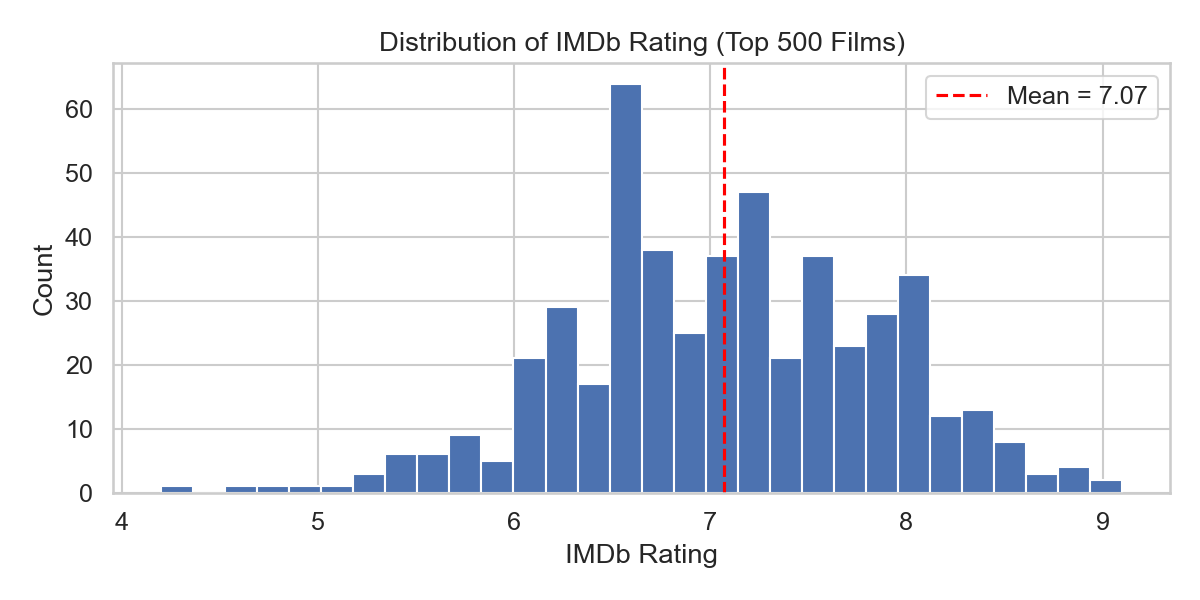
\includegraphics[width=0.78\textwidth]{../charts/eda/fig1_imdb_rating_dist.png}
  \caption{Distribution of IMDb ratings for the top 500 films.}
\end{figure}

Log-transformed domestic gross values are approximately normally distributed, with a mean of \textbf{19.26} (corresponding to $\approx$\$231M). The log transformation substantially reduces the right skew present in raw gross values.

\begin{figure}[H]
  \centering
  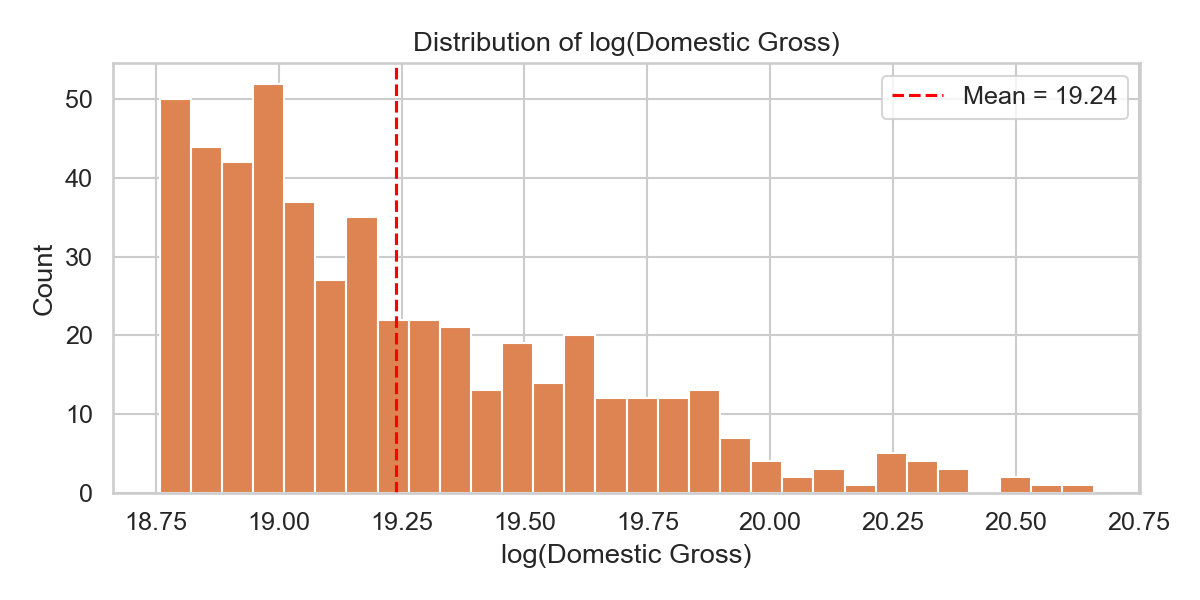
\includegraphics[width=0.78\textwidth]{../charts/eda/fig2_log_gross_dist.png}
  \caption{Distribution of log(Domestic Gross).}
\end{figure}

\subsection{Genre}

Genre is the most important categorical predictor. Action films make up the largest share of the top 500 (258/500, 51.6\%), followed by Adventure (123), Comedy (53), and Drama (32). Drama films have the highest mean IMDb rating among genres with at least 10 films in the sample, while Action and Comedy films cluster near the overall mean. Biography films underperform commercially relative to Action despite their higher IMDb ratings.

\begin{figure}[H]
  \centering
  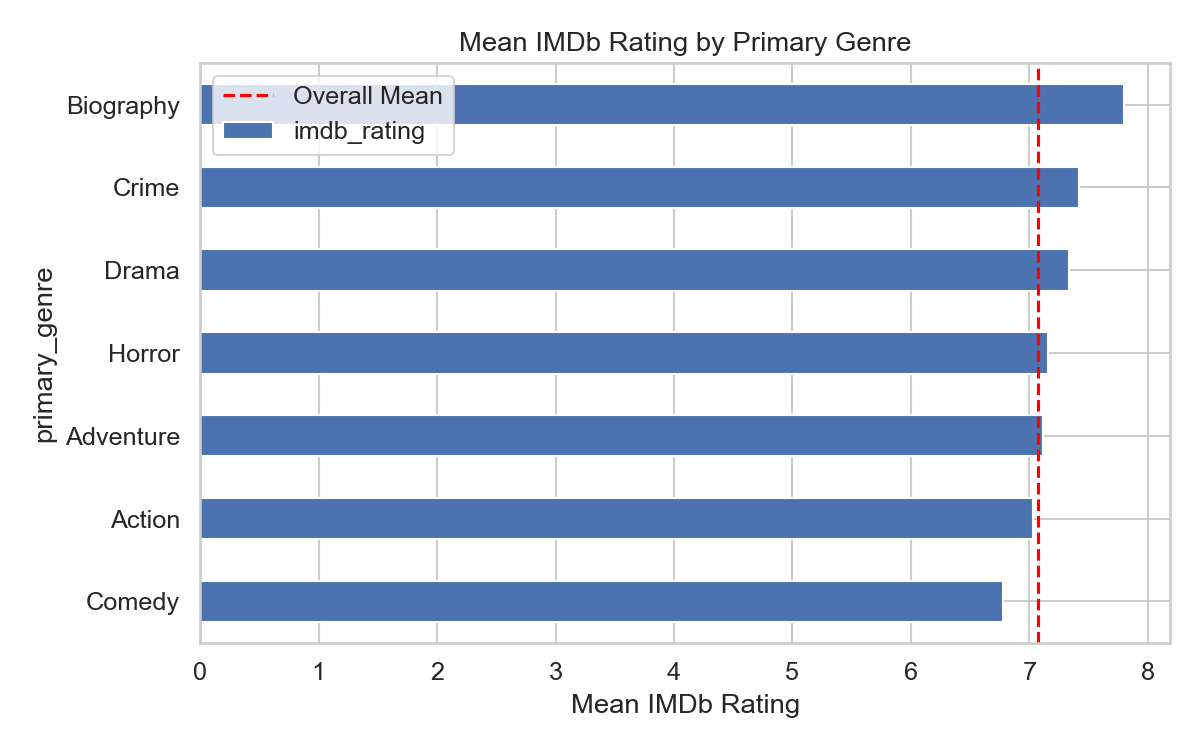
\includegraphics[width=0.78\textwidth]{../charts/eda/fig6_imdb_by_genre.png}
  \caption{Mean IMDb rating by primary genre (genres with $\geq$10 films).}
\end{figure}

\subsection{Runtime}

Runtime is the strongest continuous predictor of both outcomes:
\begin{itemize}
  \item Correlation with IMDb rating: $r = 0.27$
  \item Correlation with log(gross): $r = 0.25$
\end{itemize}

The mean runtime across all 500 films is 121.5 minutes (SD = 24.0). The positive relationship with IMDb rating likely reflects a genre confound---epic Action and Adventure films tend to be long, receive high engagement, and also earn more---rather than a direct effect of runtime itself.

\begin{figure}[H]
  \centering
  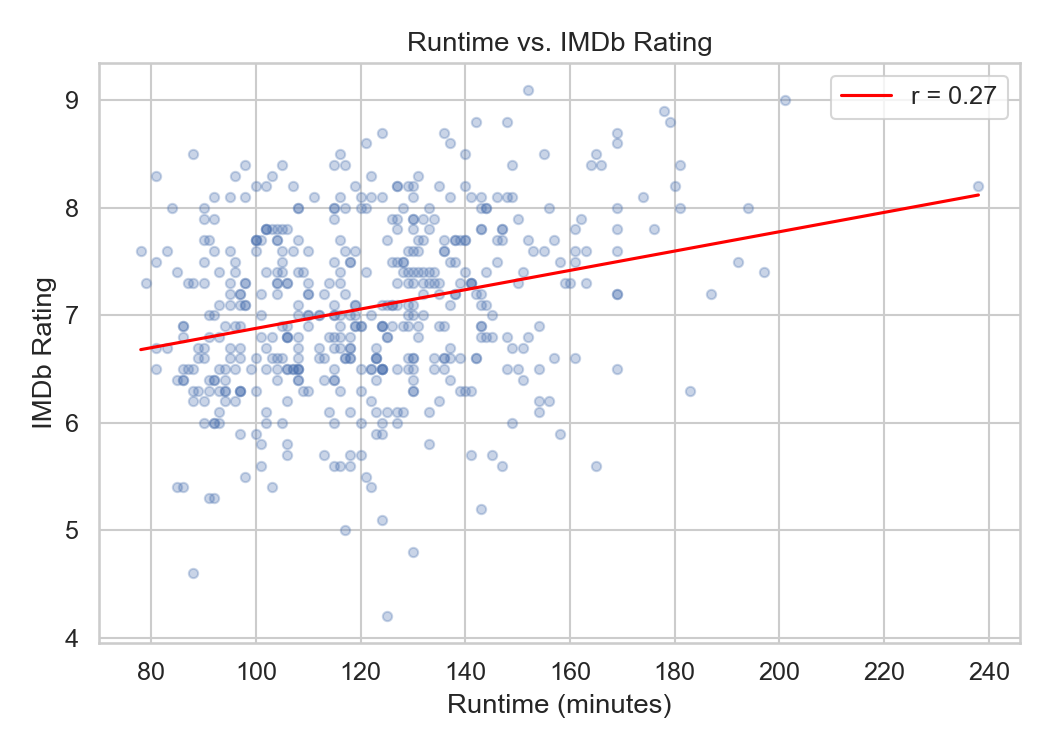
\includegraphics[width=0.78\textwidth]{../charts/eda/fig9_runtime_vs_imdb.png}
  \caption{Runtime vs.\ IMDb rating with OLS trend line.}
\end{figure}

\subsection{MPAA Rating}

G-rated films have the highest mean IMDb rating (7.58), driven by classic animated films that have aged well. PG-13 is the most common rating (258 films) and earns the most at the box office on average, reflecting its broader audience reach. R-rated films earn significantly less than PG-13 films in this sample.

\begin{figure}[H]
  \centering
  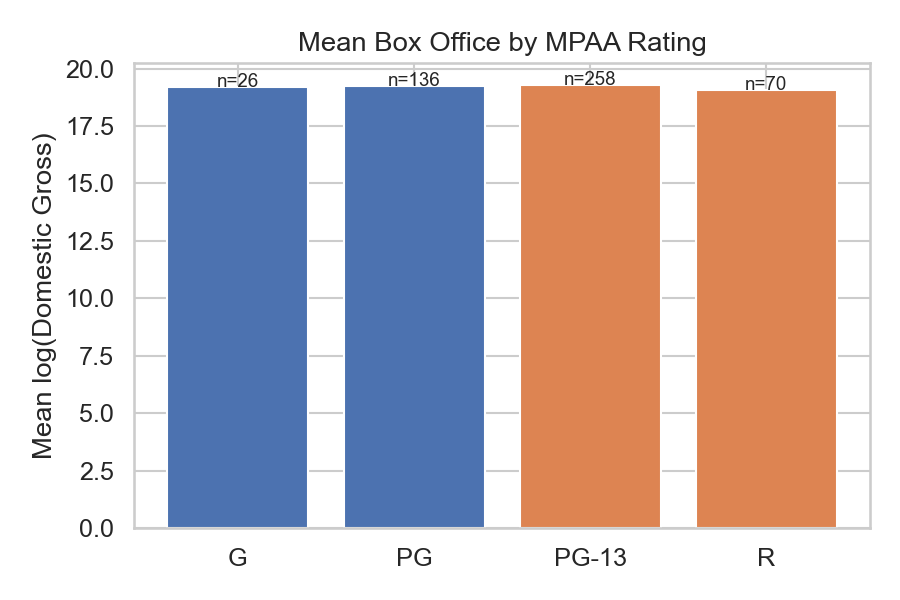
\includegraphics[width=0.72\textwidth]{../charts/eda/fig7_gross_by_mpaa.png}
  \caption{Mean log(Domestic Gross) by MPAA rating.}
\end{figure}

\subsection{Release Month}

Summer (May--July) and holiday (November--December) releases dominate the top-500 list, accounting for 289 of 492 dated films (58.7\%). January and August are the weakest months. Release month has minimal correlation with IMDb rating ($r = 0.13$) but a modest commercial association.

\begin{figure}[H]
  \centering
  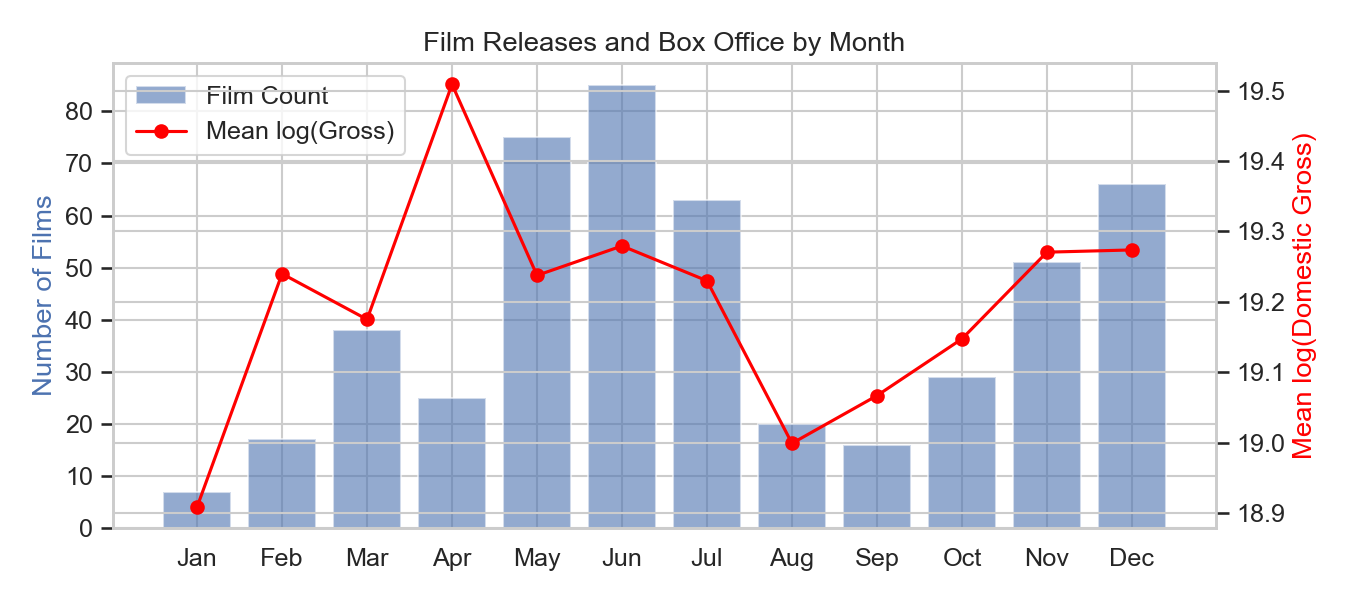
\includegraphics[width=0.82\textwidth]{../charts/eda/fig8_month_gross.png}
  \caption{Film count and mean log(gross) by release month.}
\end{figure}

\subsection{Temporal Trends}

Films from the 1970s and 1980s carry higher mean IMDb ratings than those from the 2000s and 2010s. This reflects survivorship bias: older films that remain on all-time lists have already been filtered for quality. Mean log(gross) is relatively stable across decades in nominal terms.

\begin{figure}[H]
  \centering
  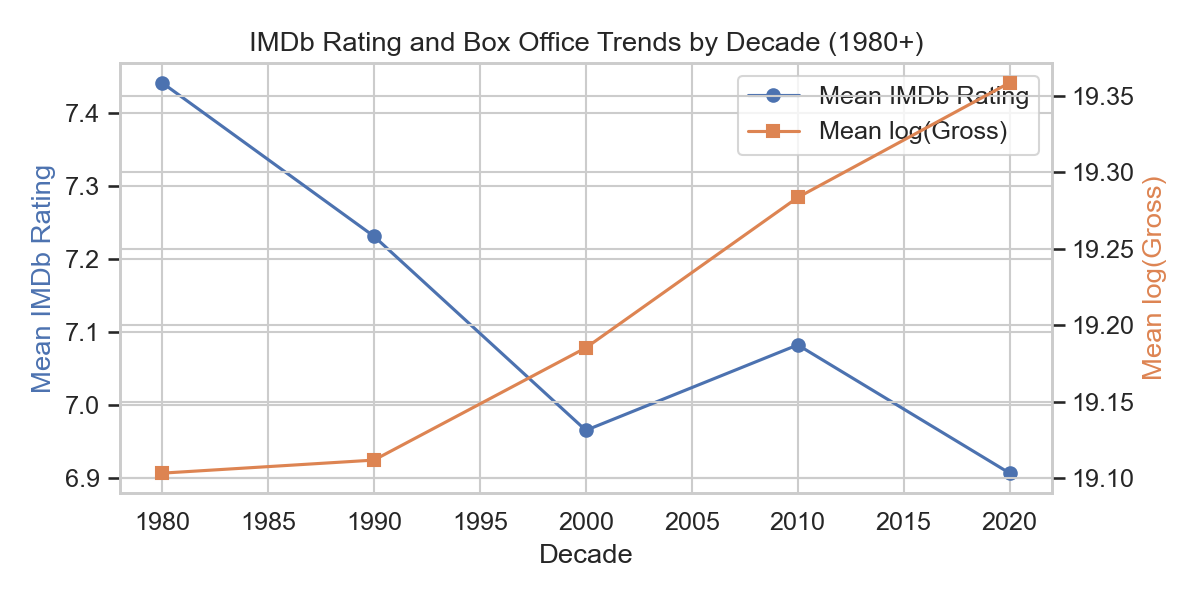
\includegraphics[width=0.82\textwidth]{../charts/eda/fig12_decade_trends.png}
  \caption{Mean IMDb rating and log(gross) by decade (1980+).}
\end{figure}

\subsection{Correlation Summary}

The heatmap below summarizes pairwise correlations among all key numeric variables. Runtime, IMDb rating, and log(gross) form a moderate positive cluster. \texttt{is\_book} has near-zero raw correlation with both outcomes. Decade has a slight negative correlation with IMDb rating and a slight positive correlation with log(gross).

\begin{figure}[H]
  \centering
  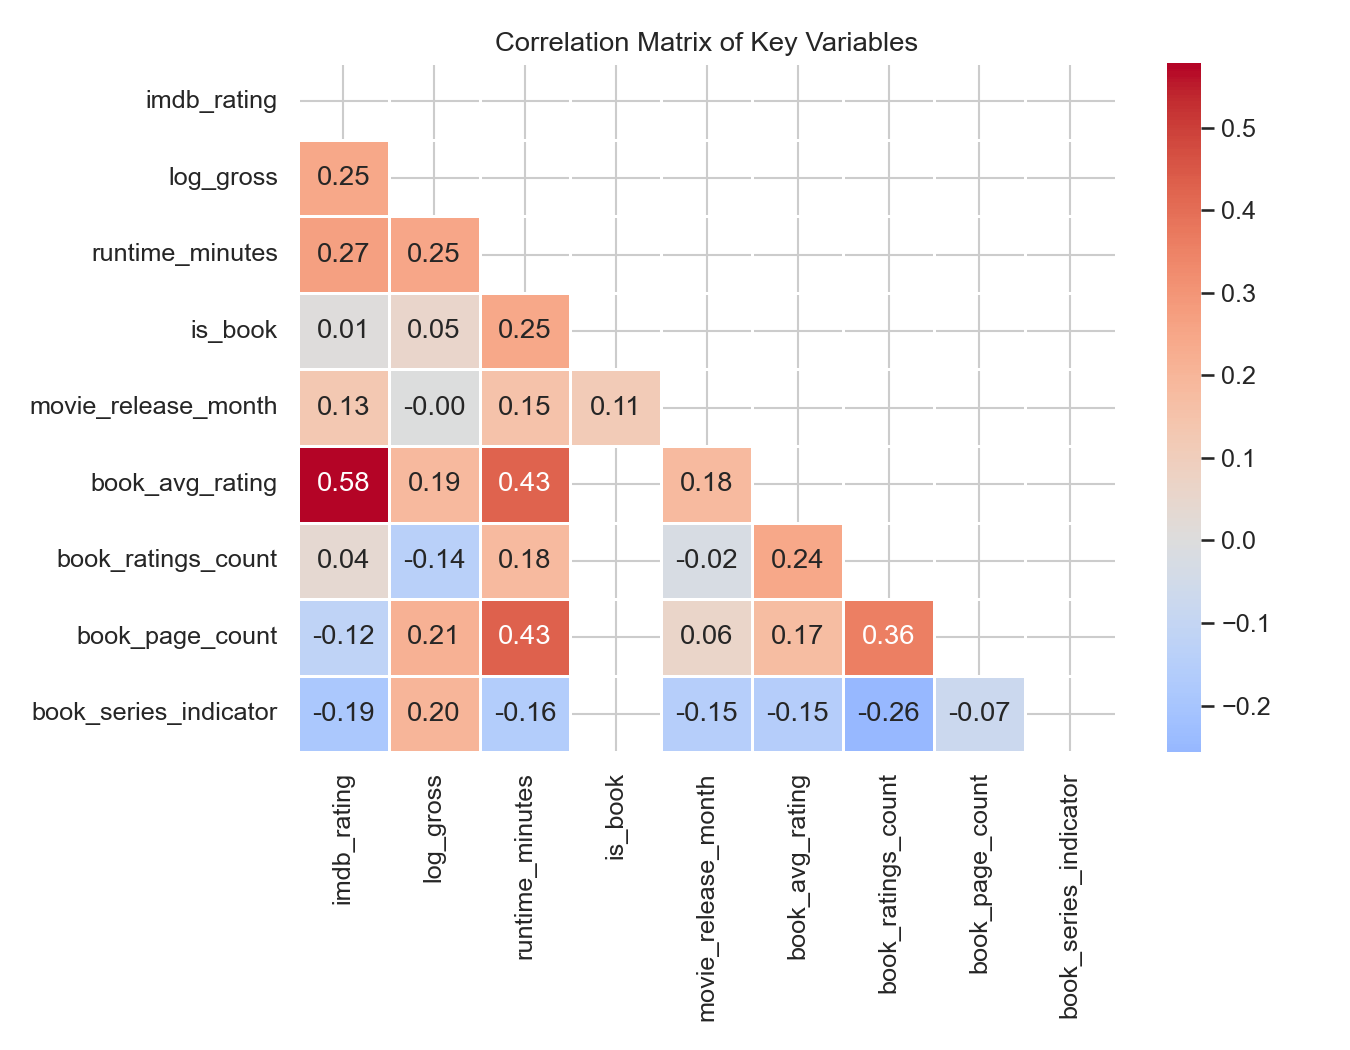
\includegraphics[width=0.88\textwidth]{../charts/eda/fig11_corr_heatmap.png}
  \caption{Correlation matrix of key variables.}
\end{figure}

%% ── Secondary: Book Adaptations ──────────────────────────────────────────────
\subsection{Book Adaptations: Exploratory Comparison}

As a secondary descriptive question, we examined whether book adaptations differ from other films in this sample.

\begin{table}[H]
\centering
\caption{Book Adaptations vs.\ Other Films}
\begin{tabular}{lrrrc}
\toprule
\textbf{Metric} & \textbf{Book (n=74)} & \textbf{Other (n=426)} & \textbf{t} & \textbf{p} \\
\midrule
Mean IMDb Rating        & 7.09  & 7.07  & 0.17 & 0.87 \\
Mean log(Domestic Gross) & 19.29 & 19.23 & 1.20 & 0.23 \\
Mean Runtime (min)      & 135.7 & 119.1 & ---  & ---  \\
\bottomrule
\end{tabular}
\end{table}

Neither difference in IMDb rating nor box office gross is statistically significant. Book adaptations do not outperform other films on either outcome before controlling for any other variables. The most notable difference is runtime: book adaptations are on average \textbf{16.6 minutes longer}, which likely reflects their genre composition (Drama: 44\% adaptations; Action: 12\% adaptations).

\begin{figure}[H]
  \centering
  \begin{minipage}{0.47\textwidth}
    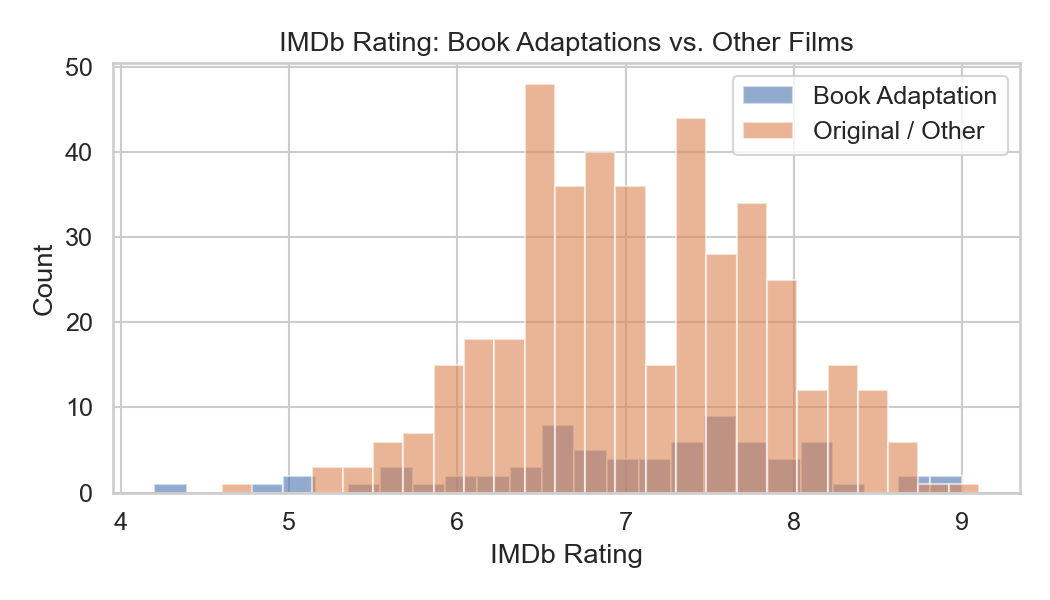
\includegraphics[width=\textwidth]{../charts/eda/fig3_imdb_book_vs_other.png}
    \captionof{figure}{IMDb rating by book status.}
  \end{minipage}\hfill
  \begin{minipage}{0.47\textwidth}
    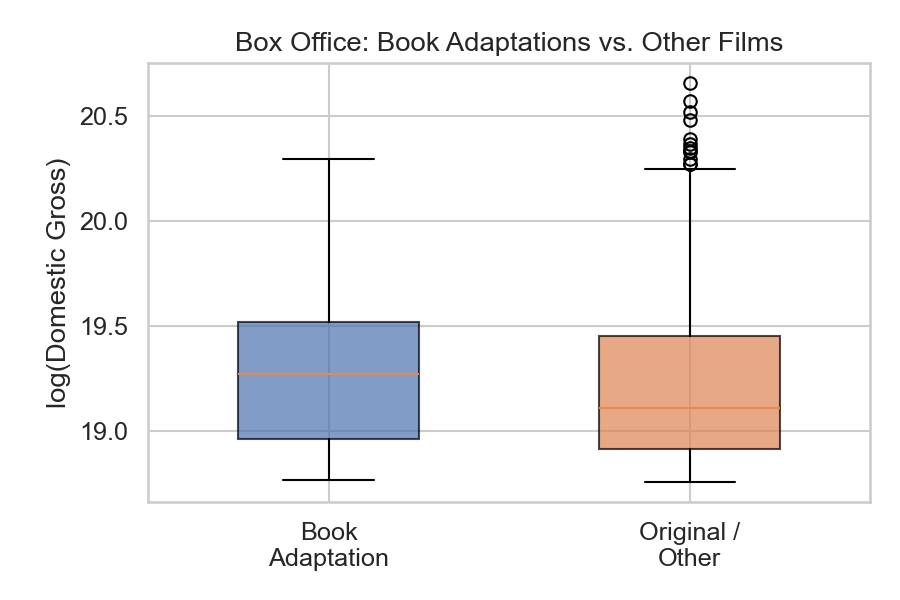
\includegraphics[width=\textwidth]{../charts/eda/fig4_gross_boxplot.png}
    \captionof{figure}{log(Gross) by book status.}
  \end{minipage}
\end{figure}

Among the 74 book adaptations specifically, Goodreads average rating shows a moderate positive correlation with IMDb rating ($r = 0.578$, $n = 73$). This suggests that the quality of the source material---as perceived by book readers---has a meaningful relationship with how the film is received by audiences. The correlation with box office is weaker ($r = 0.19$), indicating that book quality translates more to critical than commercial film reception.

\begin{figure}[H]
  \centering
  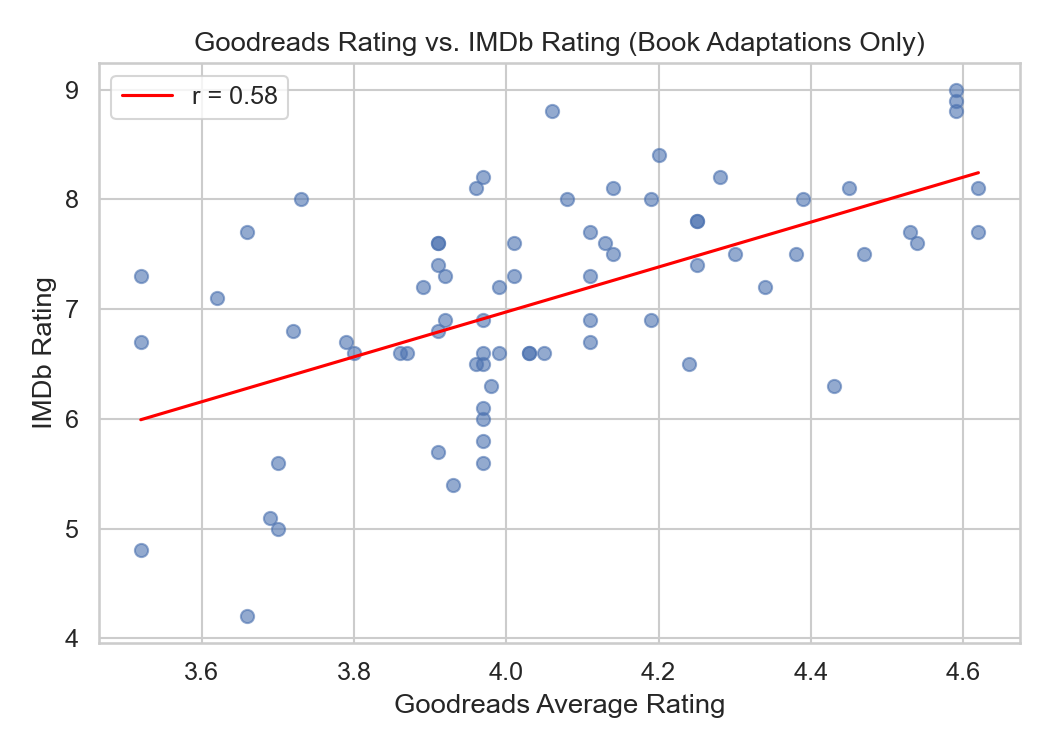
\includegraphics[width=0.72\textwidth]{../charts/eda/fig10_goodreads_vs_imdb.png}
  \caption{Goodreads average rating vs.\ IMDb rating among book adaptations ($r = 0.578$).}
\end{figure}

%% ─────────────────────────────────────────────────────────────────────────────
\section{Statistical Models}

To move beyond pairwise correlations, we fit two ordinary least squares (OLS) regression models---one predicting IMDb rating and one predicting log(domestic gross)---using the same set of film-level predictors. Genre was coded with Action as the reference category (the most common genre). MPAA rating used PG-13 as the reference. Release timing was captured via binary indicators for summer (May--July) and holiday (November--December) release windows. Runtime was included as a continuous predictor, and decade of release was included as a continuous variable to account for temporal trends.

After listwise deletion of rows missing any predictor, the model sample consisted of \textbf{487 films}.

\subsection{Model 1: IMDb Rating}

\[
\widehat{\text{IMDb}} = \beta_0 + \beta_1 \cdot \text{Runtime} + \beta_2 \cdot \text{MPAA} + \beta_3 \cdot \text{Genre} + \beta_4 \cdot \text{Summer} + \beta_5 \cdot \text{Holiday} + \beta_6 \cdot \text{Decade}
\]

\begin{table}[H]
\centering
\caption{OLS Regression: IMDb Rating (Reference: Action, PG-13)}
\begin{tabular}{lrrrr}
\toprule
\textbf{Predictor} & \textbf{Coeff.} & \textbf{SE} & \textbf{t} & \textbf{p} \\
\midrule
Intercept                  & 23.017 & 5.949 &  3.869 & $<$0.001 \\
Runtime (per minute)       &  0.011 & 0.002 &  6.847 & $<$0.001 \\
MPAA: G (vs.\ PG-13)      &  0.663 & 0.182 &  3.642 & $<$0.001 \\
MPAA: PG (vs.\ PG-13)     &  0.229 & 0.097 &  2.363 & 0.019 \\
MPAA: R (vs.\ PG-13)      &  0.251 & 0.105 &  2.391 & 0.017 \\
Genre: Biography (vs.\ Action) &  0.534 & 0.209 &  2.550 & 0.011 \\
Genre: Comedy (vs.\ Action)   & -0.211 & 0.119 & -1.768 & 0.078 \\
Genre: Adventure (vs.\ Action) &  0.059 & 0.103 &  0.578 & 0.563 \\
Genre: Drama (vs.\ Action)    &  0.079 & 0.144 &  0.550 & 0.583 \\
Summer release             & -0.062 & 0.079 & -0.791 & 0.429 \\
Holiday release            &  0.003 & 0.095 &  0.035 & 0.972 \\
Decade                     & -0.009 & 0.003 & -2.937 & 0.003 \\
\midrule
\multicolumn{5}{l}{$R^2 = 0.184$, Adj.\ $R^2 = 0.163$, $F(12,\,474) = 8.90$, $p < 0.001$, $n = 487$} \\
\bottomrule
\end{tabular}
\end{table}

\textbf{Interpretation:} Runtime is the most statistically significant predictor of IMDb rating---each additional minute of runtime is associated with a $+0.011$ point increase in rating ($p < 0.001$). Controlling for other factors, G-rated films rate $+0.66$ points higher than PG-13 films, and R-rated films rate slightly higher ($+0.25$) as well, which may reflect that R-rated films in the top 500 tend to be respected dramas or thrillers rather than typical genre fare. Biography films rate $+0.53$ points higher than Action films. Decade has a small negative effect: more recently released films rate slightly lower, consistent with survivorship bias in older films.

Release timing (summer or holiday) shows no significant effect on IMDb rating after controlling for other variables. The overall model explains \textbf{18.4\% of variance} in IMDb rating (adjusted $R^2 = 0.163$), which is modest but statistically significant. The compressed rating range in this top-500 sample limits the achievable $R^2$.

\subsection{Model 2: log(Domestic Gross)}

\[
\widehat{\log(\text{Gross})} = \beta_0 + \beta_1 \cdot \text{Runtime} + \beta_2 \cdot \text{MPAA} + \beta_3 \cdot \text{Genre} + \beta_4 \cdot \text{Summer} + \beta_5 \cdot \text{Holiday} + \beta_6 \cdot \text{Decade}
\]

\begin{table}[H]
\centering
\caption{OLS Regression: log(Domestic Gross) (Reference: Action, PG-13)}
\begin{tabular}{lrrrr}
\toprule
\textbf{Predictor} & \textbf{Coeff.} & \textbf{SE} & \textbf{t} & \textbf{p} \\
\midrule
Intercept                  &  7.624 & 2.966 &  2.571 & 0.010 \\
Runtime (per minute)       &  0.005 & 0.001 &  5.790 & $<$0.001 \\
MPAA: G (vs.\ PG-13)      &  0.085 & 0.091 &  0.939 & 0.348 \\
MPAA: PG (vs.\ PG-13)     &  0.057 & 0.048 &  1.188 & 0.235 \\
MPAA: R (vs.\ PG-13)      & -0.127 & 0.052 & -2.439 & 0.015 \\
Genre: Biography (vs.\ Action) & -0.316 & 0.104 & -3.025 & 0.003 \\
Genre: Comedy (vs.\ Action)   & -0.176 & 0.059 & -2.959 & 0.003 \\
Genre: Adventure (vs.\ Action) &  0.035 & 0.051 &  0.673 & 0.501 \\
Genre: Drama (vs.\ Action)    & -0.128 & 0.072 & -1.777 & 0.076 \\
Summer release             &  0.064 & 0.039 &  1.642 & 0.101 \\
Holiday release            &  0.067 & 0.048 &  1.411 & 0.159 \\
Decade                     &  0.006 & 0.001 &  3.722 & $<$0.001 \\
\midrule
\multicolumn{5}{l}{$R^2 = 0.186$, Adj.\ $R^2 = 0.166$, $F(12,\,474) = 9.05$, $p < 0.001$, $n = 487$} \\
\bottomrule
\end{tabular}
\end{table}

\textbf{Interpretation:} Runtime again emerges as a highly significant predictor---each additional minute is associated with a $+0.47\%$ increase in domestic gross ($e^{0.0047} \approx 1.005$ per minute). R-rated films earn significantly less than PG-13 films ($-12.7\%$ on the log scale), consistent with the broader audience access of lower ratings. Biography films earn approximately $-27\%$ less than Action films, and Comedy films earn $-16\%$ less---both statistically significant. Unlike the IMDb model, decade has a positive coefficient here ($+0.006$ per decade unit), reflecting nominal box office growth over time. Release timing trends positively but does not reach statistical significance after controlling for other variables.

The model explains \textbf{18.6\% of variance} in log(gross), nearly identical to the IMDb model. The two outcomes respond similarly to the same predictors, though with notable differences: MPAA rating matters more commercially (R-rated penalty), while rating level (G, R) matters more critically.

%% ─────────────────────────────────────────────────────────────────────────────
\section{Summary and Conclusions}

This analysis examined what film characteristics predict critical and commercial success among the 500 highest-grossing domestic films of all time. Key findings:

\begin{enumerate}
  \item \textbf{Runtime is the strongest predictor of both outcomes.} Longer films receive higher IMDb ratings and earn more at the box office. This effect is likely driven by genre (long Action/Adventure blockbusters dominate both lists) rather than runtime per se.

  \item \textbf{Genre shapes critical and commercial success differently.} Biography films rate highly on IMDb but underperform commercially. Comedy films earn less and rate slightly lower. Action and Adventure films dominate commercially but show no critical premium.

  \item \textbf{MPAA rating has asymmetric effects.} G- and R-rated films receive higher IMDb ratings than PG-13 films after controls, while R-rated films earn significantly less at the box office. PG-13's commercial dominance reflects its broad audience reach.

  \item \textbf{Release timing does not significantly predict success after controls.} Summer and holiday windows show positive but non-significant trends for box office gross.

  \item \textbf{Newer films rate slightly lower but gross slightly more} (in nominal terms), consistent with survivorship bias inflating older film ratings and nominal box office growth over time.

  \item \textbf{Book adaptations show no raw advantage} over other films on IMDb rating ($t = 0.17$, $p = 0.87$) or domestic gross ($t = 1.20$, $p = 0.23$). Among book adaptations, Goodreads source quality correlates moderately with IMDb rating ($r = 0.578$), suggesting that well-regarded source material tends to produce better-received films.
\end{enumerate}

Both models explain approximately 18\% of variance in their respective outcomes---modest but statistically significant. The compressed outcome range (all films are commercially successful by definition) limits achievable $R^2$. Future work will explore whether adding \texttt{is\_book} as a predictor improves model fit after controlling for genre and runtime, and whether Goodreads features add predictive value within the book adaptation subset.

\end{document}
